\subsection{Overview}
 High-level components and their interaction
 
\begin{figure}[hbt!]
\centering
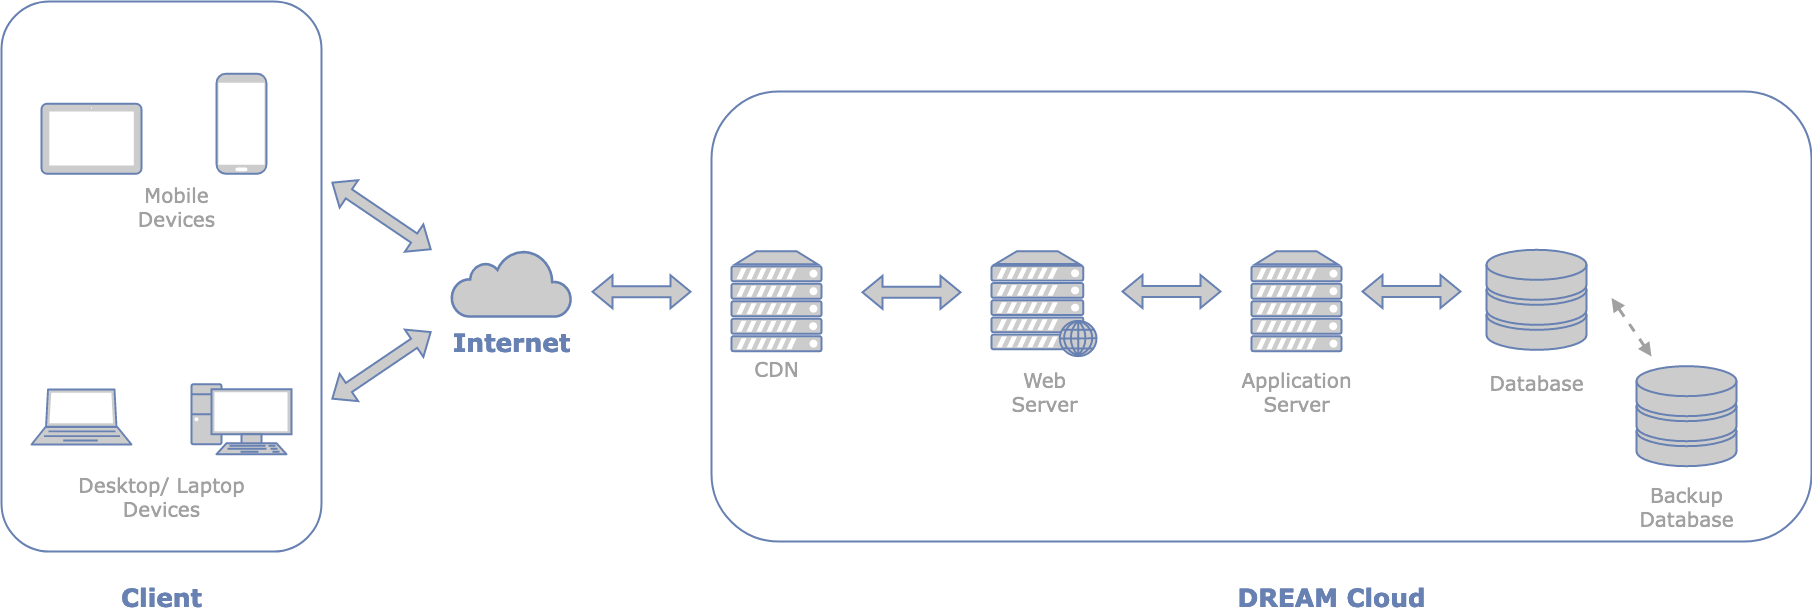
\includegraphics[scale=0.2]{../images_diagrams/dd/highlevel_arch.png}
\caption{High-Level Architecture.}
\label{fig:highLevelArch}
\end{figure}




\subsection{Component View}

\begin{figure}[hbt!]
\centering
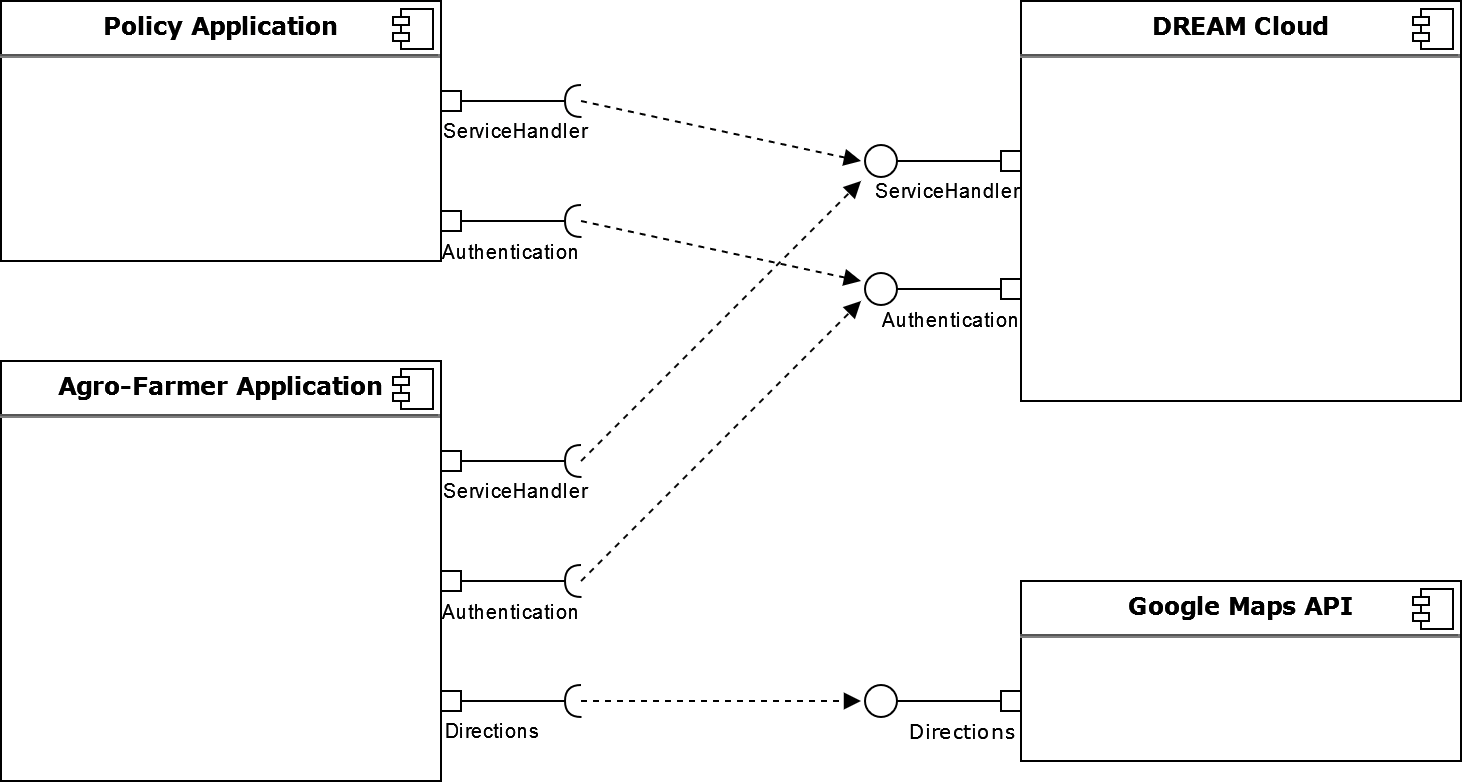
\includegraphics[scale=0.6]{../images_diagrams/dd/high_level_cloud.png}
\caption{High-Level Component View.}
\label{fig:highLevelComp}
\end{figure}

\subsection{Deployment View}
\subsection{Runtime View}
You can use sequence diagrams to describe the way components interact
to accomplish specific tasks typically related to your use cases
\subsection{Component Interfaces}
\subsection{Selected Architectural Styles and Patterns}
Please explain which styles/patterns you used, why, and how
\subsection{Other Design Decisions}